%!TEX root = ../main.tex

\chapter{相关网格简化算法及其分析}
\section{QEM 网格简化算法}
QEM算法凭着其简单高效的特点是网格简化算法中主流算法之一。在QEM算法中,每一个模型被视为是由很多个离散的有限平面所组成,而模型上的每一个顶点就是其一环邻域(周围的一圈)平面的交点。因此,我们将顶点$v=[x,y,z,1]^T$和一系列平面关联起来,相当于每一个顶点$v$都应该在一个平面集合$\text{planes}(v)$的每个平面上。每一个$\text{plane}(v)$都可以表示为$p^Tv=0,p=[a,b,c,d]^T,a^2+b^2+c^2=0即ax+by+cz+d=0$,从而该顶点到这个平面$\text{plane}(v)$的距离的平方可表示为$(p^Tv)^2$即$v^Tpp^Tv$,每一个顶点到其平面集合的距离平方和为
\begin{equation}
  \Delta(v) = \sum_{p\in \text{planes}(v)}v^Tpp^T = v^TQ_vv
\end{equation}
我们称$\Delta(v)$为Quadric Error在初始的情况下$\forall v,\Delta(v)=0$。在QEM算法中,我们用这个Quadric
Error作为简化结果与原模型的距离衡量标准。当我每做一次顶点合并$(v_0, v_1) \to v̅$时,我们将这两个顶点的平面集合合并成为新的顶点的平面集合即planes(v̅) = planes(v 0 ) ∪ planes(v 1 ),从而会产生一个新的Quadric Error$\Delta(v̅)=v^T(Qv_0+Qv_1)v$。该算法以最小化Quadric Error的上界为目标,每次都是以贪心的策略从可合并的顶点对(构成一条边的两个顶点,或者两个距离小于一定阈值的顶点)中选取$\Delta(v̅)$最小的顶点对做合并。该算法实现起来非常简单,可以归纳为以下几步:
\begin{enumerate}
  \item 初始化每个三角网格上的顶点的矩阵Q;
  \item 通过$\text{minimize} \; v̅^T(Qv_0+Qv_1)v̅$,计算每一条边的两个顶点的最优合并点$v̅$ ,以$\Delta(v̅)$作为这条边合并的代价,以此一个最小优先级队列;
  \item 迭代地从最小优先级队列中取出一个顶点对合并,然后更新这个优先级队列。
\end{enumerate}
QEM方法不仅简单高效,而且就算在大程度的简化要求下,简化结果非常好地保持了原模型的视觉效果(如图\ref{fig:qem-res})。
\begin{figure}[htbp]
    \centering
    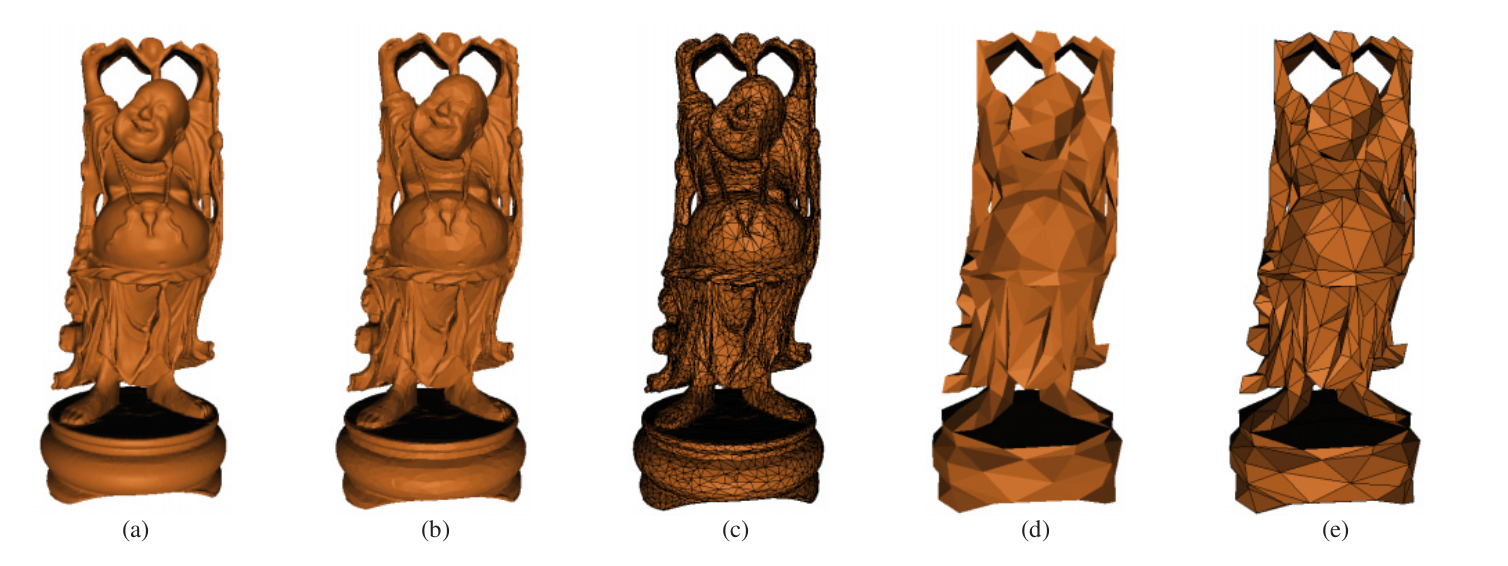
\includegraphics[width=.8\textwidth]{qem_res.png}
    \caption{使用QEM算法将模型budda从1,085,634个面(a),简化到20,000个面(b-c)和1,000个面(d-e),图来自\cite{qem2}}
    \label{fig:qem-res}
\end{figure}

\section{Memoryless Simplification 网格简化算法}
Peter Lindstrom等人在QEM算法的启发下,将$(v_0,v_1) \to \bar{v}$的Quadric Error定义为网格简化时由于顶点合并所带来的与上一步的结果之间构成的体积即:
\begin{equation}
  \Delta_1(\bar{v}) = \sum_{t_i \in \text{one\_ring}(v_0) \cup \text{one\_ring}(v_1)} \text{det} (\bar{v},v_0^{t_i},v_1^{t_i},v_2^{t_i})^2
\end{equation}
这里$t_i$是顶点$v_0$或顶点$v_1$一环邻域的三角形,$v_0^i,v_1^i, v_2^i$是这个三角形$t_i$上的三个顶点(如图\ref{fig:memory-less})。该算法相当于在标准Quadric Error的基础上,将每个平面的面积作为一个权重加入到了Quadric Error的计算中去。与此同时,当存在多对顶点的Quadric Error相同时加入了尽量保持网格质量(三角形每条边尽可能相等,不出现细长三角形)的约束,让$\bar{v}$所构成的边的平方和最小,即:
\begin{equation}
  \Delta_2(\bar{v}) = \sum_{v_i \in \text{one\_ring} (v_0,v_1)} (\bar{v}-v_i)^2
\end{equation}
\begin{figure}[htbp]
    \centering
    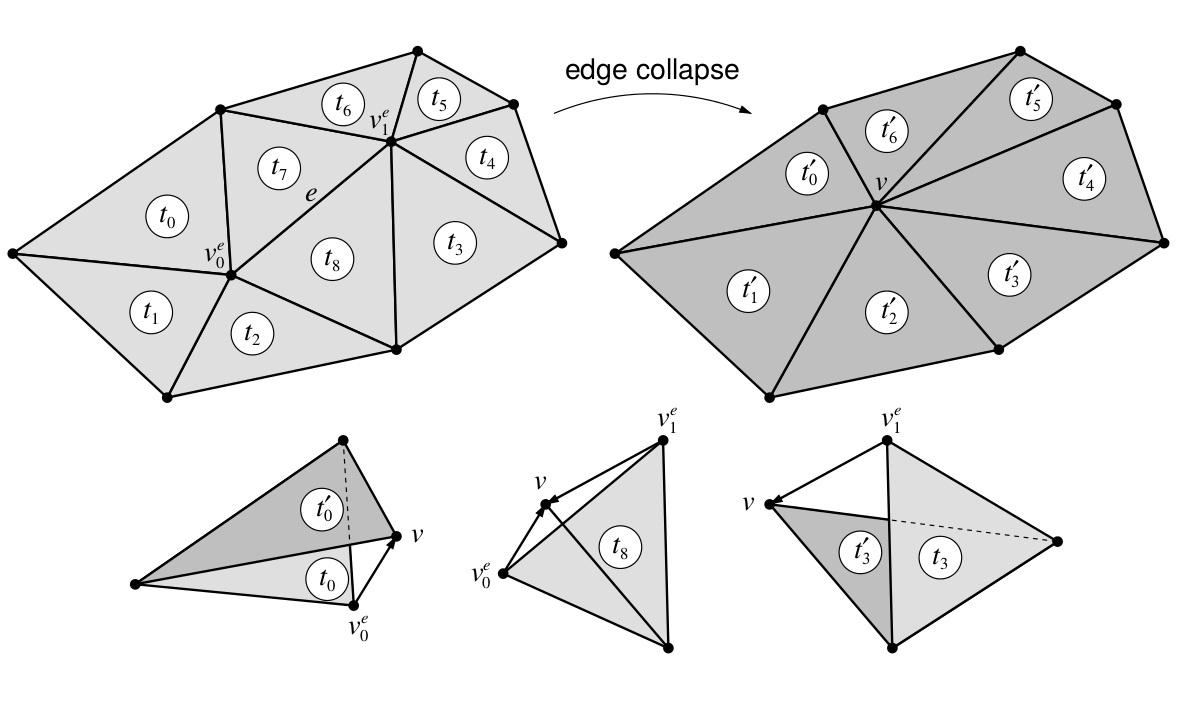
\includegraphics[width=.8\textwidth]{memory_less.png}
    \caption{顶点合并操作示意图,边e被合并到顶点v,三角形$t_7$和$t_8$在合并的过程中被删除。第二行的三个四面体显示了合并时由三角形$t_0,t_3,t_8$与合并顶点$v$所构成的体积,图来自\cite{memory-less}}
    \label{fig:memory-less}
\end{figure}
此外,该算法和QEM算法的一个很大的不同点是此方法的Quadric Error以上一次的迭代结果为计算标准,而标准的QEM的Quadric Error以初始化的网格为计算标准。从而,在相同条件下此方法通过一步步的优化迭代,该算法的结果的平均误差(平均Hausdorff距离[\ref{eq:f2f-mean-haus}])优于很多其他常用的网格简化算法,但在最大误差上逊于其他常用网格简化算法(如图\ref{fig:memory-less-compare})。
\begin{figure}[htbp]
  \centering
  \begin{subfigure}[b]{0.8\textwidth}
    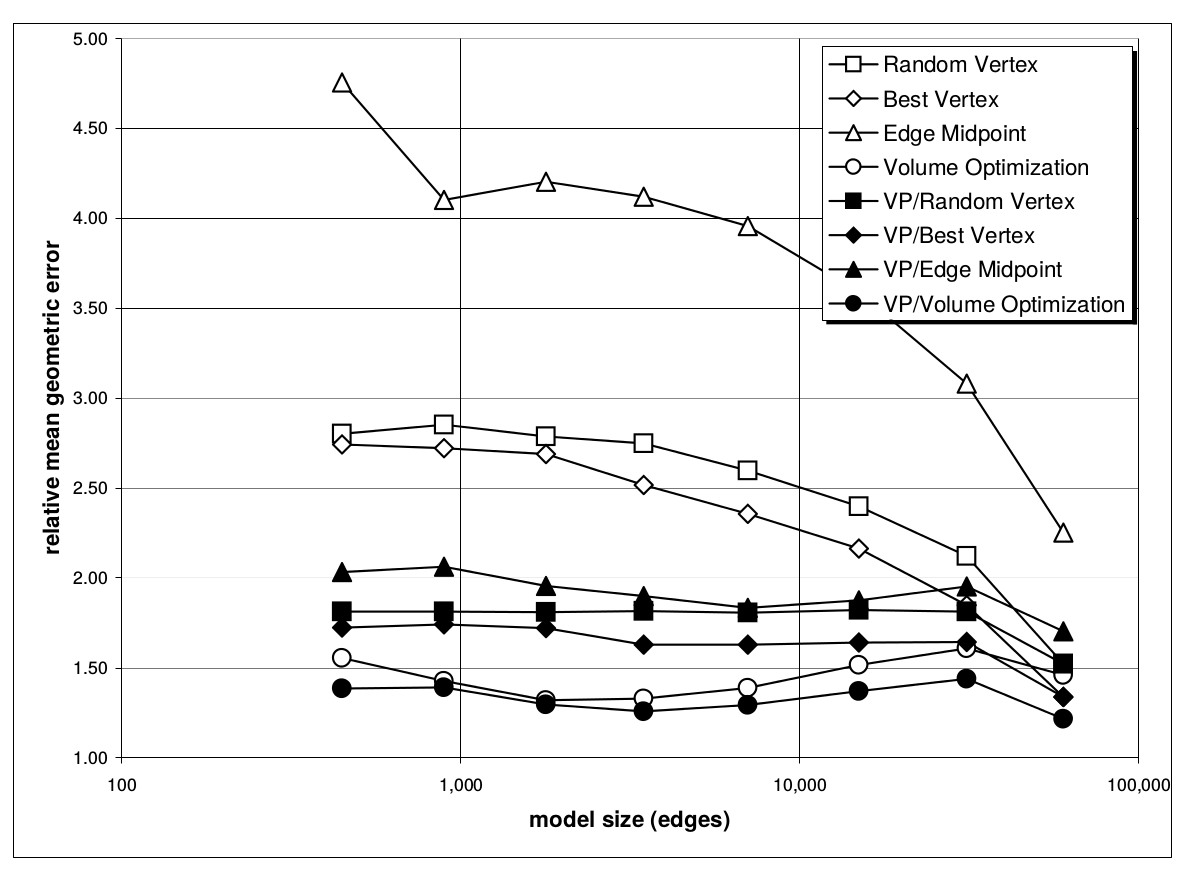
\includegraphics[width=\textwidth]{memory_less_mean_compare.png}
    \caption[input]{平均Hausdorff距离的比较}
    \end{subfigure}
    \begin{subfigure}[b]{0.8\textwidth}
      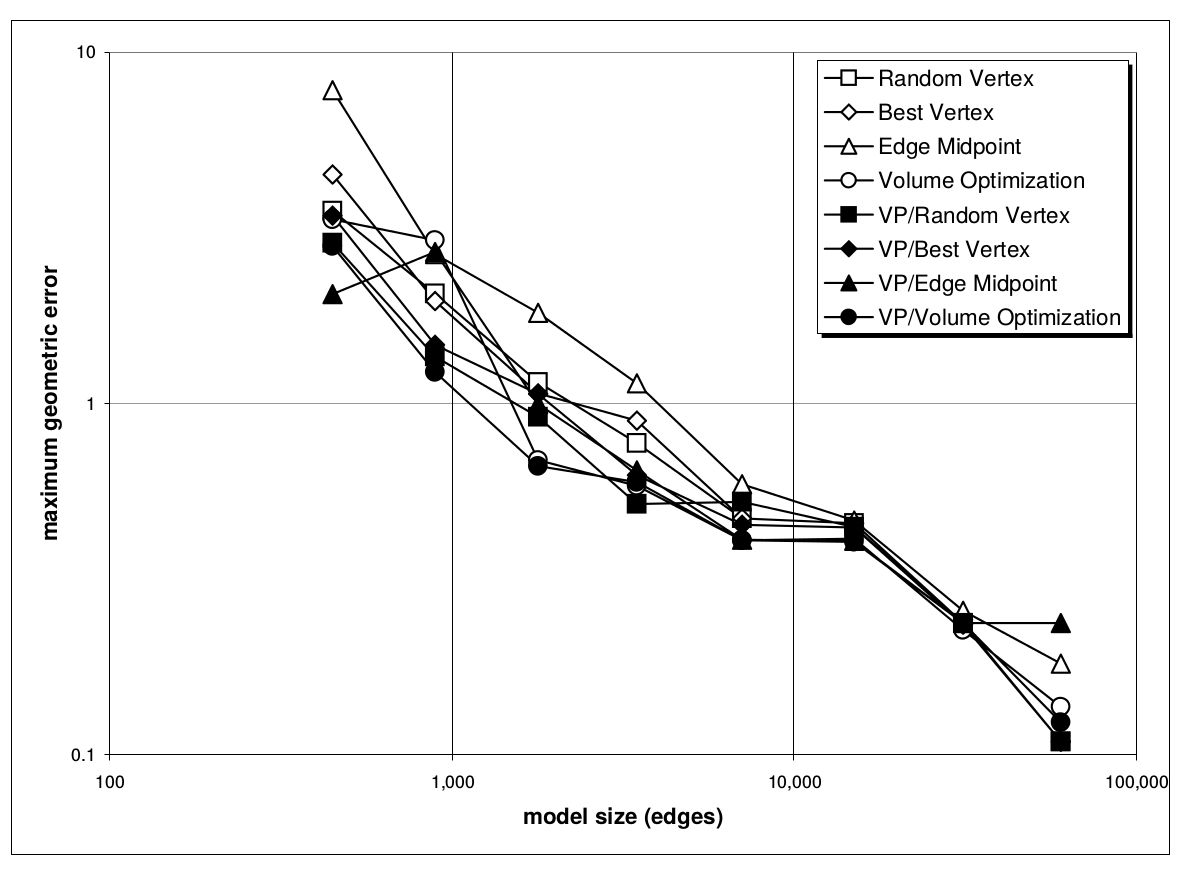
\includegraphics[width=\textwidth]{memory_less_max_compare.png}
      \caption[mls]{最大Hausdorff距离的比较}
    \end{subfigure}
    \caption[Result]{Memory Less算法在horse模型上和其他算法的简化结果的比较,图来自\cite{memory-less}}
    \label{fig:memory-less-compare}
\end{figure}
这两个算法都是$Min-\varepsilon$类算法,做不到严格控制与原模型之间的精度误差。

\section{Simplification Envelopes算法}
为了保证了输出结果在用户给定的误差范围内,Jonathan Cohen等人率先提出了一种基于内外壳的网格简化方法\cite{simp-envlop},对于给定的最大误差$\varepsilon$,通过构建两个与原模型距离为$\varepsilon$的内外壳,并保证简化结果与内外壳的相交来保证了精度。该算法主要分为三步:
\begin{enumerate}
  \item 根据用户给定的误差ε,构建内外壳;
  \item 遍历并尝试删除每一个顶点(生成一个洞),并尝试所有可能的补洞方法;
  \item 测试补洞后的网格是否在壳内,从而决定是否接受这次简化。
\end{enumerate}
为了保护原模型的拓扑结构,在构建内外壳时,我们需要保证内外壳既不能相交,也不能自交。为了做到这点,Jonathan Cohen等人提出了两种方案:基于分析的构建方法和基于数值的构建方法。在基于分析的构建方法(如图\ref{fig:compute-envlop0}),先为原网格的每一个三角形$t_i$,沿着每个顶点的法向构建一个上下分别$2\varepsilon$厚的棱柱$t_{p_i}$。然后判断每个棱柱$t_{p_i}$上的两个三角面片$\Delta_i$是否与其他棱柱相交,若与某一个棱柱$t_{p_j}$相交,则计算出在三角形$\Delta_i$上并处于棱柱$t_{p_j}$内的离三角形$t_j$的最近点的距离$\delta_{ij}$。做完所有这样的计算后,将对每一个三角形$t_i$的厚度设置为所有$\delta_{ij}$的最小值,即$\epsilon(t_i) = \text{min} \; \delta_{ij}$,而真正构建内外壳每个顶点沿法向移动的距离为$\epsilon(v) = \text{min} \; \epsilon(t_i)_{t_i \in  \text{one\_ring}(v)}$。而基于数值的构建方法,在刚开始时内外壳和原模型重合,给定一个沿法向移动的步长k,逐步地移动内外壳顶点直到达到给定的误差ε或者是检测到某三角形与其他非邻接三角形相交。为了得到一个更大的内外壳,在检测到相交并放弃移动内外壳一顶点时,将该顶点的步长设置为原来的$\frac{1}{2}$,继续尝试,直到该步长小于一定阈值之后再停止。当然对于每一个顶点可以选择不同的步长初始化,比如选取其一环邻域中对短的边的边长。\par
\begin{figure}[htbp]
    \centering
    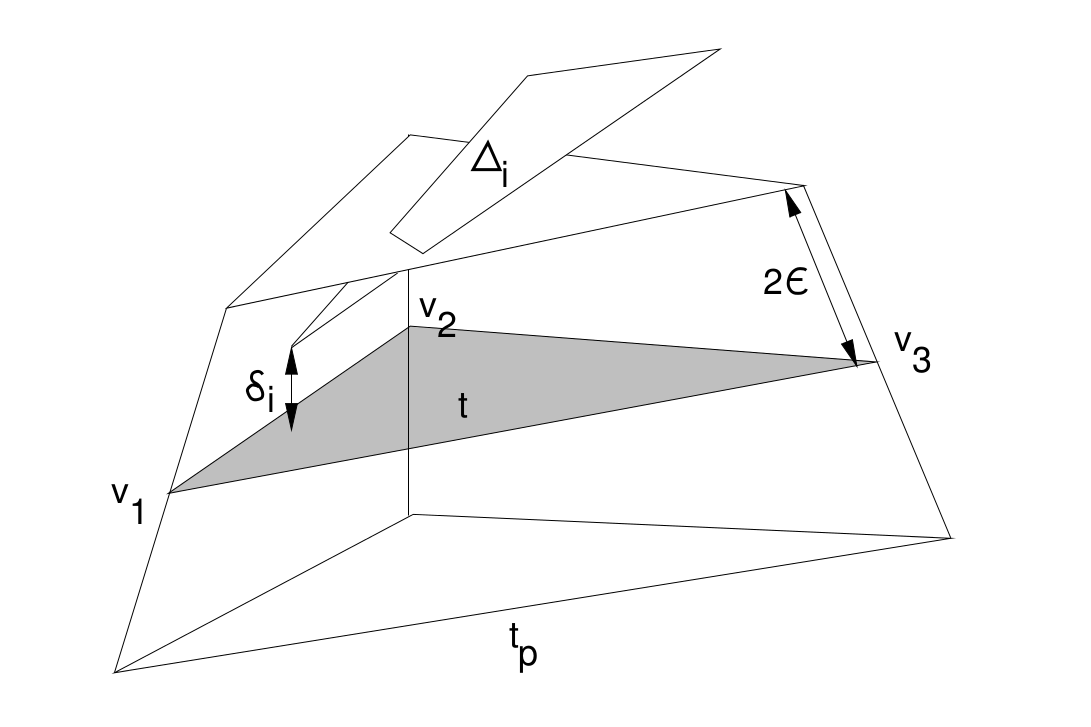
\includegraphics[width=.8\textwidth]{compute_envlop_0.png}
    \caption{基于分析的建壳方法示意图,图来自\cite{simp-envlop}}
    \label{fig:compute-envlop0}
\end{figure}
构建了内外壳之后,通过删除顶点的方式简化网格。一种简单的方式是:把每个顶点放入删除队列,然后依次送队列中取出一个顶点,尝试删除这个顶点以及其一环邻域的所有三角形,从而在原模型上产生一个洞。然后在不添加顶点的情况下,通过添加由边界点构成的三角形来补洞(有多种组合)。测试是否存在一种组合不与内外壳相交,若存在,则接受这个简化并将其邻接的顶点重新加入到队列中;若不存在,则放弃这次简化,模型保持不变。相对于尝试所有可能的补洞组合,另外一种高效的贪心补洞算法是:选取一个满足约束条件(不与内外壳相交)的三角形补上,然后递归地补上由于补上该三角形之后所产生的小的三个(或更少)的三角形。如果这种递归的补洞方法失败,则认为这个顶点删除失败即不能在保证误差的前提下通过删除这个顶点来简化网格。\par
该算法的优点是,能保证双向的Hausdorff距离在给定的误差范围内,真正做到了简化结果与原来网格之间的误差控制。而该算法的缺点也显而易见:(1)受限于内外壳不能相交这个条件,真正的$\varepsilon$不会太大,因此不能对模型做大程度的简化;(2)需要不断地做三角面片的相交检测,因此非常耗时。

\section{MMGS 算法}
从Simplification Envelopes这个算法中我们可以看到,根据用户给定的误差范围$\varepsilon$,想要鲁棒地构建一个内外壳并不那么容易,而且仅仅考虑误差,并不完全满足我们的需求。基于保证简化结果在给定的误差范围内,并且期望简化的结果尽可能光滑这两个因素,Borouchaki等人提出了MMGS算法\cite{mmgs}。该算法的主要思想是,在用户给定误差精度$\varepsilon$的条件下,通过消边的方式做模型简化,在此过程中保证简化结果和原模型之间的双向Hausdorff距离在$\varepsilon$内,并保证新生成的三角形和其周围的三角形法向基本一致(简化结果看起来比较光滑)。另外,该算法还在处理的过程中加入了翻边,和顶点移动这些模型优化方法,简化和优化迭代进行。对于模型法向的控制,与QEM算法的简化模型中法向基本一致的光滑区域的想法类似但也有所不同的是,该算法要求消除一条边PQ(将P合并到Q如图XX)之后,新生成的任意一个三角形K′的与其周围的三角形法向基本一致也即简化之后的模型尽可能光滑,K需满足:
